%%
%% INTRODUCTION
%%
\chapter{Introduction}
\label{ch:introduction}

\begin{fquote}[Jimmy Lin]Science these days has basically turned into a data-management problem. \fqsource{{Associate Professor, University of Maryland}} \end{fquote} 

\section{Machine Learning in Cancer Research}
\label{s:mlinc}

\subsection*{Cancer}
\label{ss:cancer}
Cancer (Medically: \emph {Malignant Neoplasm }) is a disease characterized by the abnormal and uncontrolled growth of cells; their ability to migrate to other parts of human body and destroy the neighboring cells and tissues~\cite{cancer}. The lack of proper care can be fatal in cancer cases. Consider, for example, some statistics: cancer caused 7.4 million deaths worldwide (13\% of the total deaths) in 2004 \cite{whofactsheet}. In the United States, cancer accounted for 0.56 million deaths (23.1\% of all deaths) in 2005~\cite{american}. Finland also has a high number of cancer cases; 26,279 new cancer cases were reported in 2007, by 2015 it is expected to reach 30,000~\cite{finnish}. It is estimated that more than one-third of the population will develop some form of cancer during their lifetime. %\cite{somethinghere}.
Cancers can appear at any age but is more common in the older population. As people have started living longer, the problems with cancer is bound to increase in the near future. As a result of the appalling effect of cancer and their growing rate, cancer is highly researched through diversified aspects and areas.

Ever since the concept of Evidence based medicine was promulgated in the early 1960s by a Scottish Professor Archie Cochrane~\cite{thatreviewarticle} in his book ``\textit{Effectiveness and Efficiency: Random Reflections on Health Services}'', a variety of different engineering tools and techniques have been used in medicine. Several ICT (Information and Communication Technologies) and computational methods such as Telemedicine, Medical imaging, Electronic Patients records have already been deployed with excellent results in hospitals and medical centers. Recently, there has been tremendous improvements in technology especially in hardware and software related to computers. Computers also have increased processing speed and storage space. Furthermore, ultramodern computer architecture, and improved communication and Internet have increased the ease of manipulation and sharing of data and resources among different communities and regions. Thus, data related to diseases, such as cancer, is efficiently stored and readily available.

On the other hand, biological systems are very complex. Technology has not only enabled storage of data, it has also provided means to study the complex biological system. Microarray technology, such as CGH (Comparative Genomic Hybridization)~\cite{cgh} and aCGH (Array Comparative Genomic Hybridization)~\cite{acgh} offer the facilities to study the genomes and the genes in human. CGH is one of the molecular techniques to survey the DNA copy number variation across the whole genome. In CGH experiment, differentially labeled test and reference genomic DNA (Deoxyribonucleic Acid) are cohybridized to normal metaphase chromosomes. Fluorescence ratios along the length of the chromosome provide a cytogenetic representation of DNA copy number variation. However, one major drawback of CGH is the resolution. The mapping resolution is only 20Mbp (Mega-Base Pairs) i.e. the smallest measurable detail is 20Mbp. In addition to that mapping resolution for deletion is 2Mbp. To overcome the problem of CGH, a new microarray technology called aCGH has been developed. aCGH provides higher resolution than CGH. Fluorescence ratios at arrayed DNA elements provide a locus by locus measure of the copy number changes. Furthermore, a type of DNA arrays called BAC arrays (Bacterial Artificial Chromosome) covers the whole genome in an overlapping manner consisting of as many BAC clones as necessary (which is $\approx$32400 for the human genome)~\cite{bacdna}. DNA arrays also includes Oligonucleotide arrays~\cite{oligo} and promoter arrays~\cite{promoter}. Oligonucleotide arrays and cDNA arrays are generally used for gene expression analysis (determining the expression level of each gene). Oligonucleotide arrays also find their application in SNP (Single Nucleotide Polymorphism) analysis. Promoter arrays are often used to identify transcription factor binding sites. Next generation sequencing~\cite{nextgen, nextgen1, nextgen2} provides an opportunity for high-throughput sequencing producing data at exponential rates. 

These technologies have varying uses including the gene expression analysis, detecting aberrations in genes and chromosomes and have a positive impact on cancer research. Furthermore, completion of the Human Genome Project~\cite{humangenomeproject, humangenomeproject1} in 2003 has opened an interesting area of research in computational genomics. The most common aspect of all these techniques is that they produce data in astronomical proportions. For instance, the third generation of DNA sequencers~\cite{nextgen1, nextgen2} will generate many petabytes\footnote{1 petabyte is equal to 1024 TB (terabytes) or 1,048,576 GB (gigabytes).} of information a year. The introduction and application of these methods in cancer research have led to the accumulation of data at exponential rates. Hence, there is an urgent need to understand complex biological systems from this huge amount of data which involves the analysis of the data exploded by those experiments. This is where a relatively new field of ML (Machine Learning) and DM (Data Mining) is increasingly finding its way in the medical field, especially in the cancer research.

\subsection*{Machine Learning and Data Mining}
\label{ss:mldm}
Machine learning is a branch of artificial intelligence incorporating a myriad of statistical, probabilistic and optimization techniques allowing computers to learn from past examples to help detect and discover meaningful patterns from large, noisy and complex data sets~\cite{mitchell, hykin, bishop}. Machine learning encompasses a variety of methods, including classification, regression, clustering, and pattern discovery with varying applications such as object recognition in computer vision, natural language processing, medical diagnosis, bioinformatics, brain-machine interfaces, classifying DNA sequences, speech and handwriting recognition. The machine learning and data mining, although a relatively new field, its community has already developed a cohort of many fascinating algorithms, interesting ways to handle the concept classes and elegant and clever ways to search through huge databases. The medical field can, therefore, reap the benefit of these methods and adapt these methods for analysis of ever increasing medical data.

Recently, machine learning methods are increasingly used in cancer research because of its versatility, the sheer volume of data generated by the biological experiments, dramatic growth in new scientific questions, and new challenges for learning and inference. The presence of massive population-wide, lifelong, trans-generational, and electronically accessible datasets obligates the use of machine learning and data mining methods in health-care and medicine. Different classification methods are used for cancer diagnosis, clustering for prognosis and tumor class discovery, and feature selection for biomarker identification~\cite{mlforcr}.  The concept of \textbf{personalized medicine}\footnote{One United States Senate Bill (proposed law) defines personalized medicine as \emph {the application of genomic and molecular data to better target the delivery of health care, facilitate the discovery and clinical testing of new products, and help determine a person's predisposition to a particular disease or condition.}}, which is essentially a set of methods to map diagnostic results to therapies in cancer cases, has led to the application of different novel machine learning methods. Furthermore, a variety of new scientific and clinical problems introduced almost everyday necessitate  the  development of novel supervised and unsupervised learning methods to use these growing resources in terms of data and knowledge. Cancer genomics is a highly researched area producing significant amount of data and questions for the research.

\section{Chromosomal Aberrations}
\label{s:chrabr}
It is important to note that cancer is a multifactorial\footnote{Here multifactorial is used to mean there are many factors causing cancer. The majority of the noninfectious diseases are multifactorial.} disease as shown in~\cite{Myllykangas200815}. For example, it is well known that smoking causes cancer, but all cancers are not caused by smoking and all the people who smoke will not develop cancer. However, all the cancer cases incorporate some form of genetic changes in human beings. Humans have 23 ~(22, X and Y) pairs of chromosomes. Humans being a diploid organism have two homologous copies of each chromosome, usually, one inherited from the father and the other from the mother. During the complex process of cell division, some abnormalities can occur in the cells and copy number changes from two~\cite{aberrations}. These changes are often referred to as CNV (Copy Number Variation). The reasons for such abnormalities have not been identified yet but even the latest studies~\cite{lateststudies} believe in the abnormality of chromosomes as a cause of cancer. It is, however, important to note that fork stalling and template switching, a replication misstep, has been attributed to such abnormalities~\cite{abnormality}. Deletion, often referred to as loss, is the case when the copy number is less than two. Duplication, often referred to as gains, is the case when the copy number is more than two. Amplification is the special case of duplication where the copy number increases more than 5. Chromosomal aberrations such as DNA amplification, deletion and duplication have significant roles in cancer research~\cite{aberrations}. Some amplifications have shown more than 100 copies. DNA copy number amplifications have been defined as the hallmarks of cancer~\cite{Tikka2007972}. 

\section{Multiple Resolutions of Genome}
\label{s:multipleresolutions}

\begin{figure}[h!]
\centering
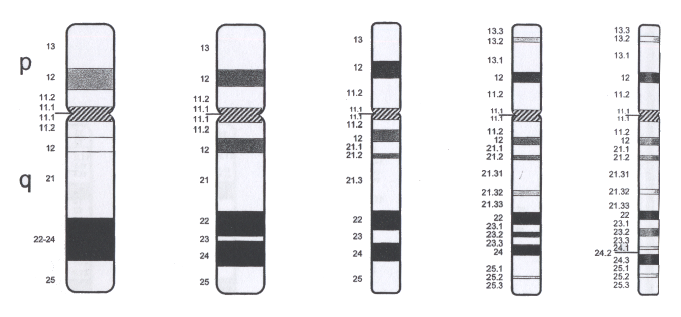
\includegraphics[width=0.95\textwidth]{figures/bands17.eps}
\caption[G-banding patterns in different resolution]{G-banding patterns for normal human chromosomes at five different levels of resolution. Source: Shaffer et. al. 2009~\cite{iscn}. Example case in Chromosome 17.} \label{Fig:probmultires}
\end{figure}

Biological experiments performed with high throughput and high resolution techniques often produce data in multiple resolutions. Furthermore, ISCN (International System for human Cytogenetic Nomenclature) has defined five different resolutions of the chromosome band: 300, 400, 550, 700 and 850~\cite{iscn}. In other words, chromosomes are divided into 862 regions in resolution 850 (fine resolution) and 393 regions in resolution 400 (coarse resolution). Figure~\ref{Fig:probmultires} shows the G-banding patterns showing five different resolutions in chromosome 17. For example, chromosome 17 in resolution 300 is divided into 10 parts while in resolution 850, the same chromosome 17 is divided into 24 different parts. Division of the regions is irregular and varied for different regions. Some regions are not divided at all where as some other regions are divided into many different parts. For example, in chromosome 17, the region 17q22 is not divided at all in resolution 400, 550, 700 and 850. However, region 17q21 is divided differently in resolutions 400, 550, 700 and 850. Furthermore, different staining techniques produce chromosome bands in different resolution. However, typically computational algorithms work with only single resolution of the chromosome. Thus, data is available in different resolutions thus necessitating new methods to be devised to work with the multiple resolutions of the data. Currently, the general principle for working in multiple resolution has been to work independently on two different resolutions and get the separate results and at best compare them. The improvement on the above principle is to transform the data to a common representation and apply the machine learning algorithm to the data in the same representation. We implement both the principles in this thesis. Furthermore, the models that directly learn from multiple resolutions of data can be developed, which is left as future work as a perspective post-graduate studies.

Working with multiple resolutions of data is important for the database integration and utilization of all the data and other available resources in multiple resolutions. Furthermore, comparing the results of an algorithm on data in different resolutions can produce interesting results which aid in determining suitable resolution of data. In addition, experiments in different resolutions can be helpful in determining the appropriate method for staining. Furthermore, machine learning and data mining algorithms and methods are in most cases data hungry and require significantly large amount of data for plausible results. Thus, database integration is important to work with high dimensional data having small number of samples. For example, the validation technique cross-validation used in this thesis has been shown not to work very well with small sized data samples in~\cite{unreliable, cvinmicroarray}. Multiresolution data occurs naturally in various fields such as telecommunication industry, image processing; thus working with multiresolution data can be interdisciplinary and signifies the importance of working with multiresolution data.

In this thesis, upsampling, a technique to transform the data from coarse resolution to fine resolution, and downsampling, a technique to transform the data from fine resolution to coarse resolution of chromosome bands, is used to transform the data in different resolutions to a single resolution which are explained in detail in Chapter~\ref{ch:sampling}. Then it presents a mixture modelling approach to reveal the structure in the chromosomal aberrations of cancer patients. The use of mixture models is motivated by the fact that cancer is not a single disease but a collective term for a class of diseases with some similarity. As the classes are different, the causes of cancers also differ among different types of cancers. Mixture models usually thrive in modeling such heterogeneous data generated from different classes. These models can be used to develop generic models to combine the samples from different sub-populations\footnote{Subpopulation is used here to mean different types of cancers. Each subpopulation represents a type of cancer}. The model based clustering approach is used to optimally divide the data into clusters. Cross-validation technique is used to learn the model i.e. the number of subpopulation that the data supports. The parameters of the mixture models are learned from the data using the Expectation Maximization (EM) algorithm~\cite{wolfe, expectmax}. The chromosomewise modeling generates a probability distribution to express the amplification patterns in cancer for each chromosome. This probability distribution can be used for the classification of different types of cancer. The chromosomal aberrations dataset analyzed in this thesis uses very scarce data as explained in Section~\ref{s:dataset}. Thus, we decided to work chromosomewise because of the availability of very few samples of the data to constrain the complexity of the mixture models.


\section{Outline of the Thesis}
\label{s:outline}
Chapter~\ref{ch:introduction} introduces the topic of the thesis with motivations for studying cancer using machine learning methods. It also provides brief introduction to the problem of chromosomal aberrations in multiple resolutions. Chapter~\ref{ch:mixturemodels} covers the mixture models, Expectation Maximization (EM) algorithm and other relevant theoretical background required for the work in the thesis. Similarly, Chapter~\ref{ch:sampling} focuses on the methods for upsampling and downsampling of chromosomal aberration data available in multiple resolutions. Chapter~\ref{ch:experiments} discusses the various experiments performed and analyzes the results of experiments. Chapter~\ref{ch:summary} draws conclusions from experimental results and discusses potential future areas of research.


\section{Contributions of the Thesis}
\label{s:contributions}
The major contributions of the thesis are briefly summarized below:

\begin{enumerate}
 \item Upsampling and downsampling methods to transform the genomic data to different resolution facilitating database integration.
 \item The chromosomewise analysis of chromosomal aberrations in multiple resolutions using mixture models of multivariate Bernoulli distributions for the data in the same resolution. 
 \item Studying the behavior of the mixture models in different resolutions.
 \item Investigation of the patterns in the multiple resolutions of data and the trained mixture models.
\end{enumerate}